%!TEX program = xelatex

\documentclass{beamer}
\usepackage{ctex, hyperref}
\usepackage[T1]{fontenc}
\usepackage{fancyhdr}%页眉页脚
\usepackage{geometry}%页面布局
\usepackage{emptypage}%空页
\usepackage{xeCJK}%中文
\usepackage{graphicx}%图
\usepackage{amssymb}%idk
\usepackage{amsmath}%idk
\usepackage{pifont}%集合符号字体
\usepackage{subcaption}%图片标题
\usepackage{picinpar}%图文
\usepackage{lastpage}%页码
\usepackage{tabularx}%等宽表格
\usepackage{array}%同上 
%\usepackage{newtxtext}%下列两个是创建颜色文本框的
\usepackage[dvipsnames,svgnames]{xcolor}
\usepackage{tcolorbox}
\usepackage{tikz}%画图
\usepackage{hyperref}%超链接
\usepackage{amsthm}%定理
\usepackage{listings}  % 用于插入代码
\usepackage{booktabs} % 三线表
\usepackage{multirow} % 表格
% \usepackage{unicode-math}


\usefonttheme{professionalfonts}
% \usefonttheme{serif}

% \usepackage[orientation=landscape,size=custom,width=16,height=9,scale=0.4,debug]{beamerposter}
% 修改 slides 比例，

% other packages
\usepackage{latexsym,amsmath,xcolor,multicol,booktabs,calligra}
\usepackage{graphicx,pstricks,listings,stackengine,cite}

\setbeamertemplate{bibliography item}[text]
\bibliographystyle{plain}
% 如果参考文献太多的话，可以像下面这样调整字体：
% \tiny\bibliographystyle{plain}

\author{ECUSTPC 2026 Spring 裁判组}
\title{2026 年华东理工大学程序设计锦标赛\\ 试题分析}
\institute{ECUST}
\date{April 7th, 2026}
\usepackage{College}

\setmonofont{Fira Code}

% defs
\def\cmd#1{\texttt{\color{red}\footnotesize $\backslash$#1}}
\def\env#1{\texttt{\color{blue}\footnotesize #1}}
\definecolor{deepblue}{rgb}{0,0,0.5}
\definecolor{deepred}{rgb}{0.6,0,0}
\definecolor{deepgreen}{rgb}{0,0.5,0}
\definecolor{halfgray}{gray}{0.55}

\newcommand{\contestbox}[2]{%
  \newtcbox{#1}{on line, arc = 0pt, outer arc = 1pt,
    colback = #2, colframe = #2,
    boxsep = 0pt, left = 3pt, right = 3pt, top = 3pt, bottom = 3pt,
    boxrule = 0pt, bottomrule = 1pt, toprule = 1pt, leftrule = 1pt, rightrule = 1pt}
}
\newcommand{\contestboxwhite}[2]{% % 文字为白色的版本
  \newtcbox{#1}{on line, arc = 0pt, outer arc = 1pt,
    colback = #2, colframe = #2, coltext=white,
    boxsep = 0pt, left = 3pt, right = 3pt, top = 3pt, bottom = 3pt,
    boxrule = 0pt, bottomrule = 1pt, toprule = 1pt, leftrule = 1pt, rightrule = 1pt}
}

\definecolor{Line1}{HTML}{FFFF00}
\definecolor{Line2}{HTML}{0066FF}
\definecolor{Line3}{HTML}{9966FF}
\definecolor{Line4}{HTML}{33CC33}
\definecolor{Line5}{HTML}{FF5050}
\definecolor{Line6}{HTML}{99CCFF}
\definecolor{Line7}{HTML}{CCCCCC}
\definecolor{Line8}{HTML}{333333}
\definecolor{Line9}{HTML}{FFCC66}
\definecolor{Line10}{HTML}{CC00CC}
\definecolor{Line11}{HTML}{CCFF66}
\definecolor{Line12}{HTML}{3DC3B6}

\contestbox{\myboxi}{Line1}   \contestboxwhite{\myboxii}{Line2}  \contestboxwhite{\myboxiii}{Line3}
\contestbox{\myboxiv}{Line4}  \contestboxwhite{\myboxv}{Line5}   \contestbox{\myboxvi}{Line6}
\contestbox{\myboxvii}{Line7} \contestboxwhite{\myboxviii}{Line8} \contestbox{\myboxix}{Line9}
\contestboxwhite{\myboxx}{Line10}  \contestbox{\myboxxi}{Line11} \contestbox{\myboxxii}{Line12}

\lstset{
    basicstyle=\ttfamily\small,
    keywordstyle=\bfseries\color{deepblue},
    emphstyle=\ttfamily\color{deepred},    % Custom highlighting style
    stringstyle=\color{deepgreen},
    numbers=left,
    numberstyle=\small\color{halfgray},
    rulesepcolor=\color{red!20!green!20!blue!20},
    frame=shadowbox,
}

\newcommand{\TT}[1] {{\ttfamily #1}}
  
\newcommand{\BF}[1] {\textbf{#1}}

\newcommand{\BS}[1] {\boldsymbol{#1}}



\begin{document}


\begin{frame}
    \titlepage
    \begin{figure}[htpb]

    \end{figure}
\end{frame}

\begin{frame}
\small
\begin{multicols}{2}
    \tableofcontents[sectionstyle=show,subsectionstyle=hide]
  \end{multicols}
    % \tableofcontents[sectionstyle=show,subsectionstyle=hide,subsubsectionstyle=show/shaded/hide]
\end{frame}

% \setmathfont{Latin Modern Math}
\section{总体}
\subsection{难度}
\begin{frame}{难度预估}
    \begin{table}[htbp]
          \large
         \begin{tabular}{cc}
          \toprule
          难度 & 题号 \\
          \midrule
     Easy & \myboxix{      \BF{\TT{I}}} \myboxvi{      \BF{\TT{F}}} \\
     EasyMedium &  \myboxvii{      \BF{\TT{G}}} \myboxii{      \BF{\TT{B}}}  \myboxx{      \BF{\TT{J}}} \\
     Medium & \myboxiv{      \BF{\TT{D}}} \myboxviii{      \BF{\TT{H}}}  \myboxxii{      \BF{\TT{L}}}  \\
     MediumHard & \myboxi{      \BF{\TT{A}}}  \myboxiii{      \BF{\TT{C}}}\\
     Hard & \myboxv{      \BF{\TT{E}}} \myboxxi{      \BF{\TT{K}}}\\
        \bottomrule       
        \end{tabular}
  \end{table}
  % \myboxix{      \BF{\TT{I}}} \myboxvi{      \BF{\TT{F}}} \myboxvii{      \BF{\TT{G}}} \myboxii{      \BF{\TT{B}}}  \myboxxii{      \BF{\TT{L}}} \myboxx{      \BF{\TT{J}}} \myboxiv{      \BF{\TT{D}}} \myboxviii{      \BF{\TT{H}}} \myboxi{      \BF{\TT{A}}}  \myboxiii{      \BF{\TT{C}}} \myboxv{      \BF{\TT{E}}} \myboxxi{      \BF{\TT{K}}}
\end{frame}

\subsection{知识点}
\begin{frame}{技巧表}
    \begin{table}[htbp]
      \begin{center}
          \large
         \begin{tabular}{cccc}
          \toprule
          题号 & 技巧 & 题号& 技巧\\
          \midrule
      \myboxix{      \BF{\TT{I}}} & 语法 & \myboxviii{      \BF{\TT{H}}}  & 计数\\
      \myboxvi{      \BF{\TT{F}}} & 讨论 & \myboxxii{      \BF{\TT{L}}} & 数学，DP\\
     \myboxvii{      \BF{\TT{G}}} & 数论，贪心 & \myboxi{      \BF{\TT{A}}} & 几何\\    
     \myboxii{      \BF{\TT{B}}} & 构造 & \myboxiii{      \BF{\TT{C}}} & 可持久化线段树\\
     \myboxx{      \BF{\TT{J}}} & 线性 DP & \myboxv{      \BF{\TT{E}}} & 图论，线性 DP \\
     \myboxiv{      \BF{\TT{D}}} & 交互，图论 & \myboxxi{      \BF{\TT{K}}} & 构造\\
      \bottomrule       
        \end{tabular}
      \end{center}
  \end{table}
\end{frame}


{
\setbeamercolor{frametitle}{fg=black, bg=Line9}

\section[I]{Problem I — 星露谷物语}
\subsection{I 星露谷物语}

\begin{frame}{题意概述}

\begin{center}
试题 \myboxix{      \BF{\TT{I}}} \BF{星露谷物语}
\end{center}
有两种类型的多种作物，每个作物属性不同：

\begin{itemize}
  \item 成本 $p$ 金，售价 $q$ 金，需要 $t$ 天成熟的一次性作物；
  \item 成本 $p$ 金，售价 $q$ 金，需要 $t$ 天成熟，后每 $s$ 天可以收获一次的多次成熟作物。
\end{itemize}

计算在 $k$ 天的春季中在一块耕地上利润最大的作物能收获的利润。

\end{frame}


\begin{frame}{贪心}

对于单次收获作物，设其能完成 $x$ 个种/收循环，$1 + xt \le k$, 可得 $x$ 最大为 $x = \lfloor \frac{k - 1}{t} \rfloor$, 因此利润为 \[\left\lfloor\frac{k - 1}{t}\right\rfloor \cdot (q - p).\]

对于多次收获作物，首先由于 $t \le k - 1$ 一定至少能长成一次。

设其能完成 $y$ 个收获循环，$1 + t + ys \le k$, 可得 $y$ 最大为 $y = \lfloor \frac{k - 1 - t}{s} \rfloor$, 因此利润为 \[\left(\left\lfloor \frac{k - 1 - t}{s} \right\rfloor + 1 \right)q - p.\]

计算所有作物的利润，加上 $0$ 取个最大值即可。

复杂度 $\mathcal{O}(n + m)$.

\end{frame}

}


{
\setbeamercolor{frametitle}{fg=black, bg=Line6}

\section[F]{Problem F - 迷路日}
\subsection{F 迷路日}




\begin{frame}{题意概述}

\begin{center}
试题 \myboxvi{      \BF{\TT{F}}} \BF{迷路日}
\end{center}

欧氏平面上的小人从给定位置出发，初始朝某个方向，只能前进一格或右转 $90^\circ$。
求她最少需要右转多少次，才能到达目标位置。

\end{frame}


\begin{frame}{分类讨论}

可以发现最多只要转 $3$ 次就可以了，有很多做法，这里列举一个简单的讨论方法。

记 $\boldsymbol{f}$ 为初始的前进单位向量，$\boldsymbol{g}$ 为顺时针转 $90^\circ$ 后的前进单位向量，$\mathrm{d}x = x_l - x_t$, $\mathrm{d}y = y_l - y_t$.

我们计算下面两个变量，本质上是把最终坐标旋转归一到标准坐标系，其中 $\langle \cdot, \cdot \rangle$ 表示内积：

\[
  a = \langle (\mathrm{d}x, \mathrm{d}y), \boldsymbol{f} \rangle, b = \langle (\mathrm{d}x, \mathrm{d}y), \boldsymbol{g} \rangle.
\]
随后画图可以看到，当然也可以严格证明：

\begin{itemize}
  \item 答案为 $0$ : $a \ge 0$, $b = 0$;
  \item 答案为 $1$ : $a \ge 0$, $b > 0$;
  \item 答案为 $2$ : $a < 0$, $b \ge 0$;
  \item 答案为 $3$ : $b < 0$.
\end{itemize}


\end{frame}

}







{
\setbeamercolor{frametitle}{fg=black, bg=Line7}

\section[G]{Problem G — 朝复习}
\subsection{G 朝复习}

\begin{frame}{题意概述}

\begin{center}
试题 \myboxvii{      \BF{\TT{G}}} \BF{朝复习}
\end{center}

给出若干场有关赛制的比分（类似 CS），求是否存在一个合法的赛制参数使得这些比分是合法的。

\end{frame}


\begin{frame}{n, m 取值分析}

我们首先可以观察到，胜者的比分 $w_i$, 一定满足 $1 + n + k \cdot m$ 的形式，两两做差能说明 $m$ 对胜者合法当且仅当其为 $\gcd(|a_i - a_j|)$ 的因数，这个可以通过取相邻项的差求出。

我们下面从败者角度，说明 $m$ 恰好取 $\gcd(a_i - a_j)$ 是最优的：

\begin{itemize}
  \item 可以发现加时情况下比分差会落在 $[2, m + 1]$ 之间，那 $m$ 尽可能取大是不劣的。
\end{itemize}

此时钦定所有胜者中比分最小 $w_1$ 的没有进行加时同样是优的：
\begin{itemize}
  \item 可以发现不进行加时的情况下对应败者可以取 $[0, w_1 - 2]$, 这个区间是极宽的，而且加时与否仅仅影响胜方比分 $w = w_1$ 的情况，其他情况和这个无关。
\end{itemize}

\end{frame}

\begin{frame}{验证}

因此记胜者比分为 $w_1$, $w_2$, $\ldots$, $w_n$, 最小值 $w_1$，取 \[
  n = w_1 - 1, m = \gcd_{2 \le i \le n}(|w_{i - 1} - w_i|).
\]

是最优的，囊括情况最多。

随后验证败者比分：
\[
  \begin{cases}
    w_i - l_i \in [2, m + 1], &w_i \ne w_1;\\
    w_i - l_i \in [2, n + 1], &w_i = w_1.
  \end{cases}
\]

每个败者比分都落在区间内即合法，瓶颈在求 $\gcd$, 总体 $\mathcal{O}(k \log W)$.

\end{frame}

}











{
\setbeamercolor{frametitle}{fg=white, bg=Line2}

\section[B]{Problem B — 回响形态}
\subsection{B 回响形态}

\begin{frame}{题意概述}

\begin{center}
试题 \myboxii{      \BF{\TT{B}}} \BF{回响形态}
\end{center}

构造\BF{两个}不同的序列满足，或报告不可能：

\begin{itemize}
  \item 是 $1$ 到 $n$ 的排列
  \item 前缀最大值减前缀最小值之和为 $k$.
\end{itemize}


\end{frame}


\begin{frame}{边界条件和贡献分析}

不难证明前缀最大值减前缀最小值的极值情况：
\begin{itemize}
  \item 最大值在第一项是 $1$ 第二项是 $n$ 取得，此时最大值为 $(n - 1)^2$;
  \item 最小值在 $\{1, 2, \ldots, n\}$ 取得，此时最小值为 $\frac{n(n - 1)}{2}$.
\end{itemize}

显然 $k$ 超出范围的都是无解的。

我们以最小值序列 $\{1, 2, \ldots, n\}$ 为基础开始构造，记 $d = k - \frac{n(n - 1)}{2}$, 可以发现，对比最大值构造，从第二项开始每一项能产生的贡献从 $n - 2$ 递减到 $0$.


\end{frame}

\begin{frame}{具体构造}

我们从 $n$ 开始倒序维护，依次将 $d$ 减去我们能提供的贡献：

\begin{itemize}
  \item 如果这一项能提供的贡献不小于剩下的 $d$ 了，那就取 $i + d$，若这项不是 $n$ 则下一项取 $n$，这样后面的贡献都是取满的，前面相较最小值构造保持一致，不产生贡献。
  \item 否则将 $d$ 减去这项能提供的贡献 $n - i$。（这只需要在前面某项取一个 $n$ 就可以取满）
\end{itemize}

这样便构造完了第一种解，超出边界的都不能构造。

第二种解直接将我们第一种解取到的 $a_i$ 变成 $n + 1 - a_i$ 就可以了，证明略去。

\end{frame}


}

















% {
% \setbeamercolor{frametitle}{fg=black, bg=Line8}

% \section[H]{Problem H - 崩碎之歌}
% \subsection{H 崩碎之歌}




% \begin{frame}{题意概述}

% \begin{center}
% 试题 \myboxviii{      \BF{\TT{H}}} \BF{崩碎之歌}
% \end{center}

% 给定 $n$ 个含有 \texttt{-} 和小写字母的原串，每次询问前你可以任意次交换相邻的 一个\texttt{-} 和一个小写字母。

% 给定 $q$ 组询问，每次给定含有 \texttt{-} 和小写字母的 $P$ 和 $S$, 询问是否存在：

% \begin{itemize}
%   \item 前缀为 $P$ 和后缀为 $S$, $P$ 和 $S$ 相交的原串。
% \end{itemize}

% \end{frame}


% \begin{frame}{Hash}

% 考虑字符串 Hash, 因为字符串 Hash 的查找和拼接是 $\mathcal{O}(1)$ 的。

% 上述的操作本质上是将 \TT{-} 取出字符串后任意插入。


% 对于每个原串用 Hash 维护一个去掉 \TT{-} 的字符串，随后记录对应的 \TT{-} 数量。

% 对于每个询问串，同样维护纯字母串，然后用字符串 Hash 找所有相等的 $P$ 后缀和 $S$ 前缀，找到后直接把对应区段的纯字母串拉出来，拼接查找对应的 \TT{-} 数是否存在即可。

% 实现上枚举每个前后缀的长度同时用另一个指针在纯字母串上移动是比较好的。 

% \end{frame}

% }


{
\setbeamercolor{frametitle}{fg=white, bg=Line10}

\section[J]{Problem J - 烈焰风暴 2}
\subsection{J 烈焰风暴 2}





\begin{frame}{题意概述}

\begin{center}
试题 \myboxx{      \BF{\TT{J}}} \BF{烈焰风暴 2}
\end{center}

给定 $n$ 个怪物的 HP 值 $a_i$，每次可以进行如下的两种操作：

\begin{itemize}
  \item 选定一只怪物对其造成 $x$ 点伤害，消耗 $a$ 点法力值。
  \item 对所有怪物造成 $y$ 点伤害，消耗 $b$ 点法力值。
\end{itemize}

求消灭所有怪物所需的最小法力值。

$n, x, y, a, b \le 2 \times 10^6, a_i \le 10^7$.

\end{frame}


\begin{frame}{只用火球术？}

考虑维护一个 $cnt_i$ 数组，$cnt_i$ 表示 HP 为 $i$ 的怪物数量，维护 $cnt$ 的一个后缀和 $suf_i$.

我们首先考虑只用火球术，每个怪物要用的火球术数量即为 $\lceil\frac{h_i}{x}\rceil$, 用后缀和表示即为

\[
  f(0) = suf_{0} + suf_{x} + \ldots + suf_{\max\lceil\frac{h_i}{x}\rceil} = \sum_{i = 0}^{i \le \max \lceil\frac{h_i}{x}\rceil} suf_{ix}.
\]

其中 $f(m)$ 我们记为对怪物造成了 $m$ 点 AOE 伤害所需的火球术数量，上面的技巧用到了拆分 Iverson 括号交换求和顺序的技巧。


\end{frame}

\begin{frame}{加入烈焰风暴}

我们进一步分析，如果我们造成了 $m$ 点 AOE 伤害，可以发现$f(m)$ 其实是这样的：

\[
  f(m) = suf_{x + m} + suf_{2x + m} + \ldots + suf_{\max\lceil\frac{h_i}{x}\rceil x + m} = \sum_{i = 0}^{i \le \max \lceil\frac{h_i}{x}\rceil} suf_{ix + m}.
\]

这启发我们维护 $f(m)$ 的性质，这个倒序下来维护是容易的，只要考虑计算 $f(m) = f(m + x) + suf_{m}$ 就可以了。

然后枚举使用烈焰风暴的次数 $j$ 得到

\[
  cost = j \cdot b + f(j \cdot y) \cdot a.
\]

计算最小值即可，复杂度 $\mathcal{O}(\max h_i)$.

\end{frame}



}





{
\setbeamercolor{frametitle}{fg=black, bg=Line4}

\section[D]{Problem D - 左灯右行}
\subsection{D 左灯右行}




\begin{frame}{题意概述}

\begin{center}
试题 \myboxiv{      \BF{\TT{D}}} \BF{左灯右行}
\end{center}

给定 $n$ 个有向四元环 $N_i - N_{i + 1} - S_{i + 1} - S_i - N_i$, 选手在交互前给出每条边的边权，随后询问 $Q$ 次点对最短路长度，确定这些环的方向。

$n \le 10^5, Q \le 3\,500$.

\end{frame}


\begin{frame}{图结构分析}

考虑到询问次数 $Q$ 很小，每次询问需要得到 $\frac{10^5}{3\,500} \approx 29$ 个 bit 信息，而最短路长度能反映的信息是一个整数，这要求我们使用高效的编码，这时使用二进制是优秀的。

接下来我们来分析图结构：

\begin{itemize}
  \item 容易发现，每个列间隔($U_i/D_i$ 到 $U_{i + 1}/D_{i + 1}$) 有且仅有一条向左/右的边。
  \item 因此如果我们要跨列移动，这些边是必然经过的。
  \item 这启发我们根据列之间的两条边 ($U_i - U_{i + 1}$ 和 $D_i - D_{i + 1}$) 是否被经过设置类似二进制的权值。
\end{itemize}

\end{frame}

\begin{frame}{具体构造}

为了让交互和图结构简单，我们这样赋值：

\begin{itemize}
  \item 首先将 $29$ 个相邻的环分为一组，编号为 $Loop_{i, 1}$, $Loop_{i, 2}$, $\ldots$, $Loop_{i, 29}$.(最后一组不足的就全部标完)
  \item 一组里面的点记为 $U_{i, 1}$ 到 $U_{i, 30}$ 和 $D_{i, 1}$ 到 $D_{i, 30}$.
  \item 我们用上边来判断，$U_{i, j} - U_{i, j + 1}$ 分别赋值 $2^0$, $2^1$, $\ldots$, $2^{28}$.
  \item 其他所有边都赋值 $0$. 
\end{itemize}

\end{frame}

\begin{frame}{性质推理}

每一组我们只询问 $U_{i, 1}$ 和 $D_{i, 30}$ 之间的最短路，观察图可以发现：
\begin{itemize}
  \item $U_{i, j} - U_{i, j + 1}$ 会被走到当且仅当这条边是向右的。
  \item 具体的构造最短路方法是：如果当前点可以向右则向右，否则一定可以通过上下 $0$ 权重边转移到可以同列可以向右的点。
  \item 直到走到了 $U_{i, 30}$ 或者 $D_{i, 30}$, 这时候即使在 $U_{i, 30}$一定可以上下转移到 $D_{i, 30}$.
  \item 因为走回头路在这个边权方案总是不优秀的，上下转移不需要代价，所以上面直接的走法一定是优秀的。
\end{itemize}

这样子一次询问可以得到一个 $2^{29}$ 的整数，对照边按位处理即可得到方向。

至多需要 $3\,449$ 次操作，因为 $3\,449 \times 29 = 100\,021$.

\end{frame}

}




















{
\setbeamercolor{frametitle}{fg=white, bg=Line8}

\section[H]{Problem H - 朝复夕}
\subsection{H 朝复夕}

\begin{frame}{题意概述}

\begin{center}
试题 \myboxviii{      \BF{\TT{H}}} \BF{朝复夕}
\end{center}


对于给定的置换，求所有交换两个元素一次之后置换的阶数之和。

\end{frame}


\begin{frame}{LCM 和操作分类}

首先将置换拆成长度为 $L_1$, $L_2$, $\ldots$, $L_k$ 的不交轮换，初始情况阶数为 $\text{lcm}\{L_i\}$, 阶数只和这些不交轮换有关。

我们考虑不同的操作，操作分为两种：

\begin{itemize}
  \item 操作 S 是交换同一个轮换内的两个元素。
  \item 操作 M 是交换不同轮换之间的两个元素。
\end{itemize}

记 $cnt_i$ 为长度为 $i$ 的轮换数量。

\end{frame}

\begin{frame}{操作 S}

一次交换在同一个长度为 $L$ 轮换，且两个元素在这个环内距离为 $d$ 的操作，会分裂出 $L - d$ 和 $d$ 两个轮换，记这个操作为 $S(L, d)$.

因为阶数只和轮换长度有关考虑，因此所有的 $S(L, d)$ 操作是等价的。

可以发现，因为 $\sum L = n$, 而 $d \le L$, 因此枚举所有的可行的 $S(L, d)$ 的枚举次数是 $\mathcal{O}(n)$ 的。

避免重复枚举，我们这时候只讨论 $2d \le L$ 的情况，因为 $2d > L$ 时的操作 $(i, j)$ 直接取反得到 $(j, i)$ 就可以归类到一种 $2d \le L$ 的等价情况。

所有等价的 $S(L, d)$ 操作的个数即为
\[
  ops(S, L, d) = \begin{cases}
    L \cdot cnt_L, &2d < L;\\
    \frac{L}{2} \cdot cnt_L, & 2d = L.
  \end{cases}
\]

\end{frame}


\begin{frame}{操作 M}

一次交换在不同的两个长度为 $a$ 和 $b$ 的两个轮换中的元素，会合并出 $a + b$ 一个轮换，记这个操作为 $M(a, b)$.

同理所有的 $M(a, b)$ 操作是等价的。

因为轮换长度种类是至多 $\mathcal{O}(\sqrt n)$ 的，因此枚举所有可行的 $M(a, b)$ 是 $\mathcal{O}(\sqrt{n}^2) = \mathcal{O}(n)$ 的。

避免重复枚举，我们这时候只讨论 $a \le b$ 的情况。

所有等价的 $M(a, b)$ 操作的个数即为
\[
  ops(M, a, b) = \begin{cases}
    cnt_a \cdot cnt_b \cdot a \cdot b, &a < b;\\
    a^2 \cdot \binom{cnt_a}{2} , & a = b.
  \end{cases}
\]

\end{frame}


\begin{frame}{最后计算}

可以发现本质不同的操作其实是 $\mathcal{O}(n)$ 的，因此对每种操作进行计算即可。

而每种操作本质上是往 lcm 集合中插入/删除了 $\mathcal{O}(1)$ 个数，因此可以直接对每种素因子 $p_i$ 维护一个记录幂指数 $P_i$ 的 \TT{std::multiset}, 随后直接操作素因子幂指数集合往里面 \TT{insert} 和 \TT{erase} 幂指数即可，lcm 即为这些素因子取最大幂指数乘方再乘起来，也即 \[
  \text{lcm}\{L_i\} = \prod p_i^{\max P_i}.
\]

不过因为我们只需要维护前 $\mathcal{O}(1)$ 个幂指数, 因此用一个 $\mathcal{O}(1)$ 的线性表维护也是可行的，最后我们需要用栈再把操作 rollback 回来。

总体是 $\mathcal{O}(n\omega(n))$ 的，其中 $\omega(n)$ 表示不同的质因子个数，在数据范围内近似常数。

\end{frame}


}





{
\setbeamercolor{frametitle}{fg=black, bg=Line12}

\section[L]{Problem L — 海底捞月}
\subsection{L 海底捞月}

\begin{frame}{题意概述}

\begin{center}
试题 \myboxxii{      \BF{\TT{L}}} \BF{海底捞月}
\end{center}


对给定 $x$ 进行下面的操作分别至多 $a_1$, $a_2$, $a_3$, $a_4$ 次:

\begin{itemize}
  \item A: $x \leftarrow \lfloor 10\sqrt{x} \rfloor$;
  \item B: $x \leftarrow \lfloor 0.7x + 30 \rfloor$;
  \item C: $x \leftarrow \lfloor 1.2x \rfloor$;
  \item D: $x \leftarrow x + 5$.
\end{itemize}

求能得到的最大 $x$.

$T \le 10^5$, $n \le 100$, $a_i \le 400$

\end{frame}


\begin{frame}{预处理 Stage 1}

指出一些有用的事实，证明从略：
\begin{itemize}
  \item $100$ 以上前两种操作都是不优秀的，因为分数会越弄越少。
  \item 这四种操作至多 $9$, $11$, $19$, $20$ 次就会一定达到前两种操作不优秀的情况，称之为达到门槛。
  \item 通过交换可以证明 C 操作一定是最后的。
\end{itemize}

考虑设计状态 $dp_{a, b, d, x}$ 表示至多使用 $a$ 次 A 操作，$b$ 次 B 操作，$d$ 次 D 操作的前提下，$x$ 能达到的最高分。

上限分别只需要开到上面的 $a \le 9$, $b \le 11$, $d \le 20$ 即可，转移从略。

因为 C 的最后性，最后的答案是 \[
  C^{(a_3)}(\max_{0 \le d \le \min\{a_4, 20\}}\{dp_{a_1, a_2, x, d} + 5(a_4 - d)\}).
\]



\end{frame}

\begin{frame}{预处理 Stage 2}

现在我们做到了单组 $\mathcal{O}(20 + a_3)$ 了，我们尝试优化到 $\mathcal{O}(1)$.

考虑优化两个部分：

\begin{itemize}
  \item \[\max_{0 \le d \le \min\{a_4, 20\}}\{dp_{a_1, a_2, x, d} + 5(a_4 - d)\}\] 完全可以提一个 $5a_4$ 出来，然后记\[
    maxDp_{a_1, a_2, x, D} = \max_{0 \le d \le D}\{dp_{a_1, a_2, x, d}  - 5d \}.
  \]
  这样省掉了一个 $20$ 的循环。
  \item 因为 $C^{(a_3)}(a)$ 后面的定义域不超过 $2\,100$, 上面的 $a_3$ 不会超过 $400$, 直接打表预处理就可以了。
\end{itemize}

这样就做到了单组 $\mathcal{O}(1)$, 当然这个题可能有些优化不是必要的，数据范围开的不紧（单组 $\mathcal{O}(1)$ 有点难造）。

\end{frame}


}















{
\setbeamercolor{frametitle}{fg=black, bg=Line1}

\section[A]{Problem A - 聚光灯下}
\subsection{A 聚光灯下}

\begin{frame}{题意概述}

\begin{center}
试题 \myboxi{      \BF{\TT{A}}} \BF{聚光灯下}
\end{center}

给定欧氏平面上 $n$ 个中心在 $(x, y)$ 半径为 $\sqrt{x^2 + y^2}$ 的圆，找出所有圆交集中距离原点最远的点，并求出距离。

\end{frame}

\begin{frame}{先说结论}

先说结论：

\begin{itemize}
  \item 记这些圆心构成的凸包为 $K$.
  \item 答案即为原点到凸包的最短距离 $d$ 的两倍 $2d$.
\end{itemize}

还有一种做法是反演后用半平面交做，此处略去。

\end{frame}

\begin{frame}{一些引论}

容易发现这些圆一定过原点。

记 $C_i$ 是这些圆的圆心，记平面上任意一点为 $P = (x, y)$, 可以发现 $P$ 在圆 $C_i$ 内当且仅当 \[
  |P - C_i|^2 \le R_i^2 = |C_i|^2.
\]

此处用二维向量表示点。

展开并化简：

\[
  |P|^2 - 2 \langle P, C_i \rangle + |C_i|^2 \le |C_i| ^2 \Leftrightarrow  |P|^2 \le 2 \langle P, C_i \rangle
\]

其中 $\langle P, C_i \rangle$ 表示 $P$ 向量和 $C_i$ 向量的内积。

记这些圆心构成的凸包为 $K$, 原点到 $K$ 上最近的点记为 $C^\ast$, 我们分两步证明答案点就是 $2C^\ast$.

\begin{enumerate}
  \item 原点到 $2C^\ast$ 的连线在所有圆的交集内。
  \item 对任意其他在交集内的点有 $|C| \le 2|C^\ast|$.
\end{enumerate}

\end{frame}


\begin{frame}{引理 1  证明这个路径在所有圆的交集内 - 凸集投影定理}

我们首先证明一个 Lemma：

\begin{itemize}
  \item 对于 $K$ 内任意一点 $C$, 有：
  \[
     \langle C - C^\ast, C^\ast - O \rangle \ge 0.
  \]
  \item 取所有的 $C_i$ 消去 $O$ 展开即得 \[
    \langle C_i - C^\ast, C^\ast\rangle \ge 0  \Leftrightarrow  \langle C_i, C^\ast \rangle \ge |C^\ast|^2.
  \]
  \item 直观理解上，我们可以认为从 $C^\ast$ 前往凸集内任意一点都是和 $C^\ast$ 到 $O$ 方向相反的。
\end{itemize}

凸分析中有类似结论，这个结论被称之为 \textbf{凸集投影定理}，但我们用一个初等的证明方法证明：

利用反证法，不妨设 $\langle C_i, C^\ast \rangle < |C^\ast|^2$, 我们来尝试构造一个 $C'$ 不满足这个条件。

首先记 \[
  m = \langle C_i - C^\ast, C^\ast \rangle = \langle C_i, C^\ast \rangle - |C^\ast|^2 < 0.
\]

\end{frame}


\begin{frame}{引理 1 证明这个路径在所有圆的交集内 - 凸集投影定理}

我们在 $C_i$ 和 $C^\ast$ 连线段上取一点，这个点根据凸包性质一定在凸包内：

\[
  Q(t) = C^\ast + t(C_k - C^\ast).
\]

其中 $0 \le t \le 1$.

计算 $f(t) = |Q(t)|^2 = \langle C^\ast + t(C_k - C^\ast), C^\ast + t(C_k - C^\ast) \rangle$.

大力化简得到
\[
  f(t) = |C^\ast|^2 + 2t\langle C_i - C^\ast, C^\ast \rangle + t^2 |C_k - C^\ast|^2.
\]

我们可以得到惊人发现，一次项系数为 $m$.

这样取一个较小的 $t < \frac{2m}{|C_k - C^\ast|^2}$, 这时下降趋势是一次项占优的，可以得到 $f(t) = |Q(t)|^2 < |C^\ast|^2$.

这和 $C^\ast$ 是 原点到 $K$ 上最近的点是矛盾的。

\end{frame}


\begin{frame}{引理 1 证明这个路径在所有圆的交集内}

回到我们的 Lemma $\langle C_i, C^\ast \rangle \ge |C^\ast|^2$, 我们验证 $2C^\ast$ 是否符合在圆内的条件 $|2C^\ast|^2 \le 2 \langle 2C^\ast, C_i \rangle$, 代入得到

\[
  \text{LHS} = |2C^\ast|^2 = 4|C^\ast|^2.
\]
\[
  \text{RHS} = 2 \langle 2C^\ast, C_i \rangle = 4\langle C^\ast, C_i \rangle.
\]

消去系数 $4$ 即是我们刚刚证明的引理，不等式是成立的，因此 $2C^\ast$ 在所有圆的交集内。

由于圆是凸集，若干个圆的交集仍然是凸集，原点和 $2C^\ast$ 又都在这些圆的交集内，因此连线段也在交集内，路径总是合法的。

\end{frame}

\begin{frame}{引理 2 对任意其他在交集内的点有 $2C^\ast$ 是最近的}

我们记点 $S$ 是在所有圆的交集内的一点，我们只需证明 $|S| \le |2C^\ast|$.

可以发现 $C^\ast$ 是凸包上的一点，根据凸包定义存在一组 $\lambda_i$ 满足：

\[
    C^\ast = \sum_{i = 1}^{n} \lambda_i C_i,    \sum_{i = 1}^{n} \lambda_i = 1, \lambda_i \ge 0.
\]

由于 $S$ 是在所有圆的交集内的一点，有 $|S|^2 \le 2\langle P, C_i \rangle$.

将上面不等式每项乘上 $\lambda_i$ 求和:
\[
  |S|^2 = \sum_{i = 1}^{n} \lambda_i |S|^2 \le \sum_{i = 1}^{n} 2\lambda_i \langle S, C_i \rangle = \langle S, 2\sum_{i = 1}^{n}\lambda_i  C_i \rangle = \langle S, 2C^\ast \rangle.
\]

第二个等号是内积的线性性质。

\end{frame}

\begin{frame}{引理 2 对任意其他在交集内的点有 $2C^\ast$ 是最近的}

由 Cauchy-Schwarz 不等式，
\[
  \langle S, 2C^\ast \rangle \le 2 |S||C^\ast|.
\]

连接不等式有 \[
  |S|^2 \le 2 |S||C^\ast|.
\]

由 $|S|$ 的非负性，$|S| \le 2 |C^\ast|$.

\end{frame}

\begin{frame}{最终计算}

套用模板计算原点到凸包的最近距离即可：

\begin{enumerate}
  \item 最近点一定在边上，首先求凸包。
  \item 对于每条边求原点和连线段的夹角 $\langle \overrightarrow{AB}, \overrightarrow{AO} \rangle$, 若小于 $0$ 则说明投影在线段外面，最近点就是 $A$ 点， $\langle \overrightarrow{BA}, \overrightarrow{BO} \rangle$ 同理。
  \item 反之则投影在线段上，直接求三角形的高就是答案了：\[
    h = \frac{|\overrightarrow{OA} \times \overrightarrow{OB} |}{|\overrightarrow{AB}|}.
  \]
\end{enumerate}

\end{frame}

}






{
  \setbeamercolor{frametitle}{fg=white, bg=Line3}

\section[C]{Problem C - 星之所在}
\subsection{C 星之所在}

\begin{frame}{题意概述}

\begin{center}
试题 \myboxiii{      \BF{\TT{C}}} \BF{星之所在}
\end{center}

对于带权值的树，求 $q$ 条路径上满足出现次数大于 $\frac{len}{k}$ 的所有权值。

$\sum k \le 3 \times 10^5$.

\end{frame}

\begin{frame}{原树上问题}

我们尝试维护每个结点到根节点的路径权值信息。 我们需要查询的是：

\begin{itemize}
  \item 对于每个结点 $u$ 到树上根结点 $root$ 的路径上在 $[l, r]$ 之间的所有权值的出现次数 $f(u, l, r)$.
\end{itemize}


这个是容易用可持久化线段树实现的，底层是权值线段树，统计权值的出现次数。

而这个出现次数是满足可差分的，因此我们可以用上面的路径维护 $(x, y)$ 路径上的信息：

\begin{itemize}
  \item 维护结点 $x$ 到结点 $y$ 的路径上在 $[l, r]$ 之间的所有权值的出现次数 $F(x, y, l, r)$.
\end{itemize}

这个用树上差分实现，记 $\text{LCA}(x, y)$ 为 $x$ 和 $y$ 的最近公共祖先， $\text{F}(\text{LCA}(x, y))$ 为其父亲节点：
\begin{align*}
   F(X,Y, l, r) = f(x, l, r) &+ f(y, l, r) - f(\text{LCA}(x, y), l, r)\\
          &- f(\text{F}(\text{LCA}(x, y)), l, r).
\end{align*}

\end{frame}


\begin{frame}{可持久化线段树问题}

现在我们将问题完全转化为了可持久化线段树上的问题。

首先可以证明：

\begin{itemize}
  \item 满足条件的权值是至多 $k$ 个的。
  \item 因此我们从根节点开始遍历，由于线段树高度是 $\log n$ 的，因此我们必须经过的的路径长度是 $\mathcal{O}(k \log n)$ 的。
\end{itemize}

因此我们从根节点表示的区间 $[1, n]$ 开始：

\begin{itemize}
  \item 如果左儿子树上结点满足 $cnt_L > \frac{|S|}{k}$ 说明这个地方可能权值是一个答案，往下递归。
  \item 否则则不递归左儿子。
  \item 右儿子亦然。
  \item 直到叶子结点位置。
\end{itemize}

我们这样子只走了上面所述有可能有答案的线段树上结点，因此复杂度是完全正确的 $\mathcal{O}(\sum k \log n)$.

\end{frame}


}










{
\setbeamercolor{frametitle}{fg=white, bg=Line5}

\section[E]{Problem E - 右灯左行}
\subsection{E 右灯左行}

\begin{frame}{题意概述}

\begin{center}
试题 \myboxv{      \BF{\TT{E}}} \BF{右灯左行}
\end{center}

给定 $n$ 个有向四元环 $N_i - N_{i + 1} - S_{i + 1} - S_i - N_i$, 给出边权和环方向，询问 $Q$ 组点之间的最短路。


\end{frame}


\begin{frame}{图论观察}
  
首先这道题不打算放常数巨大的（如带一个 $6 \times 6$ 矩阵 Floyd）的线段树过。

下面的讨论以向右讨论为基础，向左的情况是完全一样的就省略了。

画图观察可以发现以下两个事实：

\begin{itemize}
  \item 从一列向右的出点 ($U_i/D_i$ 中有向右出边的那个) 向右走，走到另一列来自左的入点($U_j/D_j$ 中有从左入边的那个)，不经过重复点的情况下路径是唯一的。
  \item 我们把同向的环连在一起形成若干个极大的同向环块，同列点之间的最短路不会跨过环。
\end{itemize}

第一个结论是因为这些点都是必经点，割去任意一个我们要去的两个图就不连通。

第二个结论是因为若要离开同向环块，一定要经由跨环块列那一列的边至少两次，这一定比不上直接折返的。



\end{frame}

\begin{frame}{图论观察}
  
因此由必经点的结论，把不同列的最短路拆成三段（同列在我们下面的处理下会更简单）：

\begin{enumerate}
  \item 从起点到同列向右的出点；
  \item 起点列右出点到终点列左入点；
  \item 终点列左入店到同列终点。
\end{enumerate}


因此，我们总共需要处理两个查询，这分别对应了上面的两个性质：

\begin{itemize}
  \item 从 $i$ 列的右出点到 $j$ 列的左入点的路径，对应上面三段的第二段。
  \item 同列之间的上下转移最短路，对应上面三段的第一段和第三段。
\end{itemize}

这里同列只需要调用第二个查询就行了。

\end{frame}

\begin{frame}{查询跨列高速}
  
我们用前缀和维护这个东西。

记 $e_i$ 表示 $1$ 列出点到 $i$ 列入点的距离， $i$ 列入点是从 $i - 1$ 号环进来的。
记 $s_i$ 表示 $1$ 列出点到 $i$ 列出点的距离， $i$ 列出点是从 $i$ 号环出去的。

转移有两种：

\[
  s_i = e_i +  \begin{cases}
    0, & \text{dir}(L_i) =  \text{dir}(L_{i + 1}),\\
    \min(r_{k - 1}, l_k), & \text{dir}(L_i) \ne\text{dir}(L_{i + 1}).\\
  \end{cases}
\]
\[
  e_{i + 1} = s_i +   \begin{cases}
    u_i, & \text{dir}(L_i) =  \text{O},\\
    d_i, & \text{dir}(L_i) = \text{I}.\\
  \end{cases}
\]

这样只需要依照 \[
  s_1 \rightarrow e_2 \rightarrow s_2 \rightarrow e_3 \ldots \rightarrow e_{n - 1} \rightarrow s_{n - 1} \rightarrow e_{n}.
\]

转移即可，可得 $i$ 列右出点到 $j$ 列左入点代价即为 $e_j - s_i$.

\end{frame}

\begin{frame}{同列转移}

记 $f_i$ 为 $i$ 列从 $N_i \rightarrow S_i$ 的南下最短路，记 $g_i$ 为 $i$ 列从 $S_i \rightarrow N_i$ 的北上最短路。

此处我们每次只讨论一个环方向相同的连续段，按照方向是 O 处理，I 的情况是完全类似的，故略去。我们来用线性 DP 处理。

此时北岸只能东行而南岸只能西行，因此我们计算 $f_i$ 从东向西也即 $i$ 从大到小递推处理，注意第 $i$ 列左边是 $i - 1$ 环右边是 $i$ 环：

\[
  f_i = \min \begin{cases}
    r_{i - 1}, &i > 1;\\
    u_i + f_{i + 1} + d_i, &i < n.
  \end{cases}
\]

同理：
\[
  g_i = \min \begin{cases}
    l_i, & i < n;\\
    d_{i - 1} + g_{i  - 1} + u_{i - 1}, &i > 1.
  \end{cases}
\]


\end{frame}

\begin{frame}{收尾}

最后我们把上面三个查询计算加起来就行了，注意我们需要预处理双向的情况。

\end{frame}


}


{
\setbeamercolor{frametitle}{fg=black, bg=Line11}

\section[K]{Problem K - 净化行动 2}
\subsection{K 净化行动 2}

\begin{frame}{题意概述}

\begin{center}
试题 \myboxxi{      \BF{\TT{K}}} \BF{净化行动 2}
\end{center}

无限大中国象棋棋盘上存在若干固定的黑卒和一个黑将，任意部署红炮并按炮规则移动，确定能否击杀黑将。


\end{frame}


\begin{frame}{引理 1 - 行上的棋子性质}
  
我们首先研究单行上的性质。

首先定义一个自由点是和无穷远处联通的点，所有自由点都是相互连通的。随后定义一个接下来会用到的概念可击杀行（表述方便此处用行讨论，列是同理的）：

\begin{itemize}
  \item 我们首先选择这个单行上的任意一个棋子 $X_i$.
  \item 一个行是可击杀行当且仅当对于任意 $X_i$, 我们可以通过下面的操作吃掉 $X_i$ ，称其为通过该行击杀 $X_i$:
    \begin{itemize}
      \item 选择一个该行的一个点 $k$, 部署红炮。
      \item 仅能在本行吃子，或移动到一个同行的自由点。
      \item 吃完除了 $X_i$ 之外的棋子后仍能移动到一个自由点。
    \end{itemize}
  \item 特别的，如果 $k$ 是自由点，我们称其为自由击杀行。
\end{itemize}


我们指出引理 1:

\begin{itemize}
  \item 该行棋子数不为 $1$ 或 $3$ 时，则该行一定是可自由击杀的。
  \item 该行棋子数为 $3$ 但这三个棋不连续时，该行一定是可击杀的。
\end{itemize}



\end{frame}

\begin{frame}{引理 1 - 行上的棋子性质}
  
我们来证明这个引理（记 \texttt{C} 为炮，\texttt{X} 为黑方棋子，目标棋子为 \texttt{T}, 空格为 \texttt{O}）：

\begin{itemize}
  \item 棋子数量为 $2$ 时 直接选择对向部署的一个无穷远处吃掉即可 \texttt{CXT -> OXC}).
  \item 棋子数量为 $4$ 时 经由下面的操作可以吃掉第 $2$ 个和第 $4$ 个： (\texttt{CXXXX -> OXCXX -> OX.XC}), 由对称性可以得到另一边的解法。
  \item 棋子数量不少于 $5$ 时，可以进行任意次以下的操作来消灭 $3$ 个棋子：\texttt{CXXXXXX... -> OXCXXX...-> OXOXCXX... -> OCOXOXX...}
  \item 任意次操作后棋子只会剩下 $2$/$3$/$4$ 个，剩 $3$ 个的情况用对称性换成剩下另一边的三个。
\end{itemize}

三个不连续时选择中间的空地部署吃掉一边就变成 $2$ 个了(\texttt{XCXX -> XOXC}).

\end{frame}

\begin{frame}{引理 2 - 结网}
  
先把和将同一行或同一列的棋子加入集合 $S$, 接着对新加入的棋子做同样的操作，不断扩展，直到集合 $S$ 不再增加新的棋子。

我们接下来的引理 2 是：

\begin{itemize}
  \item 若 $S$ 中的棋子其所在行/列有可击杀的行/列，则可以通过一系列操作击杀将。
  \item 因此若答案要是 \texttt{NO},  $S$ 中所有的行列的棋子数量需要是 $1$, 或者是紧密相邻的 $3$ 个棋子。
\end{itemize}

我们首先如下建模：将 $S$ 中的棋子其所在行/列抽象为若干图上结点 $R_i$ 和 $C_i$, 将存在 $S$ 中棋子的交叉点 $(R_i, C_j)$ 对应的 $R_i$ 和 $C_j$ 连一条边。




\end{frame}

\begin{frame}{引理 2 - 结网}
  
可以发现图一定是联通的，因此如果存在可击杀的行/列一定存在下面的的一条路径连到将所在的行/列：

\[
  R_1 - C_1 - R_2 - C_2 \ldots - R_{\text{K}}
\]

其中我们此处令后面的行列都是不可被直接击杀的，这只需要我们选一条极短的就可以了。

由于后面都是不可被直接击杀的，因此我们从 $R_1$ 开始首先通过 $R_1$ 击杀 $(R_1, C_1)$, 这时候后面的 $C_1$ 因为本来是 $3$ ($1$ 没法和两个 $R$ 连), 击杀后会变为可自由击杀，反复操作即可击杀 $R_\text{K}$.

上面的操作第一步要求是可击杀的，后面要求可自由击杀。


\end{frame}


\begin{frame}{引理 3 - 网状结构}
  
来到第三部分，我们首先来说明一个事实：

\begin{itemize}
  \item 如果一行有 $3$ 个连续棋子，若位于中间的棋子上下没有棋子的话那这行也是可自由击杀的（中间的棋子在被击杀后是自由点）
  \item 进一步，如果上下两个棋子不是紧密相邻的话那连通块内一定有可击杀列，从而答案是 \TT{NO}.
\end{itemize}

第三步我们需要说明：

\begin{itemize}
  \item 若答案是 \texttt{NO} 连通块内的每行/列的棋子数量分布一定形如 $\{1, 3, 3, \ldots, 3, 1\}$, 且这些行/列是相邻的，内部也是相邻的。
\end{itemize}

相邻是因为如果中间有空行那一定跨越了至少一对同列的棋子，上面的论述已经表明了这个情况一定是可击杀的。

我们分两步证明若答案是 \texttt{NO} 的行数量分布：

\begin{itemize}
  \item 第一个一定是 $1$, 后面一定是一个 $3$.
  \item $3$ 后面若还有 $3$ 中间一定没有 $1$.
\end{itemize}

\end{frame}


\begin{frame}{引理 3 - 网状结构}
  
第一个若是 $3$, 可以发现这个 $3$ 的中间棋子上面无棋子，这违背了我们先前的事实，这行是可任意击杀的。

如果开头是两个 $1$, 讨论这两个 $1$ 在同列或不在同列：

\begin{itemize}
  \item 同列的情况下这列一定下面还要有一个 $1$, 但中间的 $1$ 左右又无棋子了，该列会被击杀。
  \item 不同列的话第一个 $1$ 根据上面的引理要么下边跨着空行连着另一个棋子要么干脆就不连通，都和题目条件矛盾。
\end{itemize}

再考虑如果 $3$ 后面有一个 $1$ 再后面若还有行的话：

\begin{itemize}
  \item 这时候 $1$ 一定位于 $3$ 中间的棋子下面，同时 $3$ 上面还有一个, 因此 $1$ 这一列是满的，因此后面每一列要么就是已经满 $3$ 个要么就是有空行了，因此这也是矛盾的。
\end{itemize}

\end{frame}

\begin{frame}{最终结论}
  
我们最后来看到底能构造出什么情况才能构造出一个 \TT{NO} 的答案：

从第二行的 $3$ 开始，可以发现第一行的 $1$ 一定在这个 $3$ 的中点上方。

下一行的 $3$ 需要占据第中间列，但整体一定要往左或往右偏移一格，因为下面的情形是不合法的：

\TT{.X.}

\TT{XXX}

\TT{XXX}

因为这里会发现第三行左右两边的 \TT{X} 下面都需要一个棋子，但中间的 \TT{X} 下面不可以有棋子，这就导致第四行的棋子不连续，这不合法。 


\end{frame}

\begin{frame}{最终结论}
  
也就是棋子需要长这样：

\TT{..X.}

\TT{.XXX}

\TT{XXX.}

但接下来的偏移都需要是同向的，因为可以发现上面的第三列此时已经满了，而第二列还需要一个棋子，因此每行摆放是固定的。

最后会形成这样的结构：

\TT{...X.}

\TT{..XXX}

\TT{.XXX.}

\TT{XXX..}

类似在第二列最下方摆上最后一个 $1$ 即可，这时候就构造出了合法的 $S$, 同时列也是合法的。

这样我们就构造出了唯一可能的合法情况，注意将一定在每行/列的两侧，而不是中间。

\end{frame}

\begin{frame}{实现}
  
考虑 BFS 扩展 $S$, 随后记录行列是否符合下面的规律：

\begin{itemize}
  \item 行列计数符合 $\{1, 3, 3, \ldots, 3, 1\}$, 中间无空行。
  \item 每行每列棋子连续。
  \item 偏移方向符合条件。
  \item 将不在中间。
\end{itemize}


\begin{figure}[htbp]
   \centering
   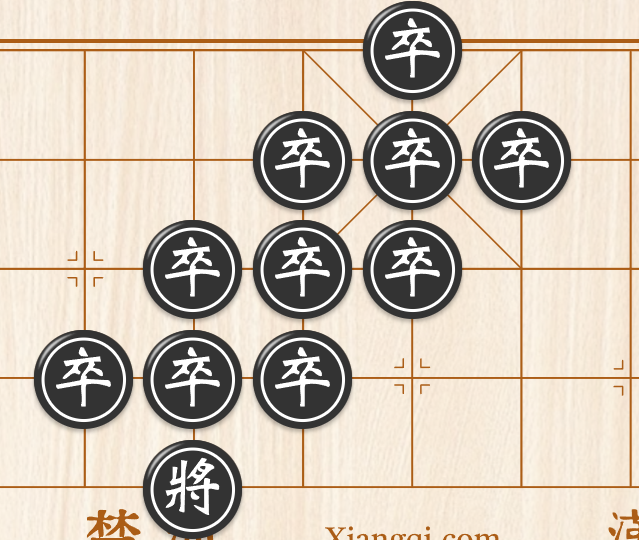
\includegraphics[scale = 0.25]{K_5.png}
   \caption{一个合法的情况}
\end{figure}


\end{frame}



}






\section*{End}

\begin{frame}{Thanks}

命题：Zhu Chenxuan (tumu1t), Ding Wenhan(pheonix\_2002), Jing Ziyun(cold\_beans)

% 验题：Buffett, KethDeorge, Lezy233, yy1120, Tony\_Zou, [数据删除]

{\center \Huge Thanks!}

\end{frame}









\end{document}
